\documentclass[a4paper]{article}

\usepackage{listings}
\usepackage{xcolor}
\usepackage{hyperref}
\usepackage{graphics}
\usepackage{graphicx}
\usepackage{geometry}
\usepackage{algorithm}
\usepackage[noend]{algpseudocode}
\usepackage{amsmath}
\geometry{margin=1.5in}
\usepackage[english]{babel}
\usepackage{url}
\usepackage{titling}

\setlength{\droptitle}{-2em}

\title{EnGPar - Partitioning Strategy for XGCM}

\author{Gerrett Diamond}

\date{\today}

\begin{document}

\maketitle

\section{Important Questions}
\begin{enumerate}
\item Are the safe zones defined as an integer amount of the flux faces? (Assumed yes)
  {\color{red}
    \begin{itemize}
    \item No, but the idea below has been altered to allow general safe zones.
    \end{itemize}
  }
\item Do the particles have computational or communication dependencies on one another? (Assumed no)
  {\color{red}
    \begin{itemize}
    \item No
    \end{itemize}
  }
\end{enumerate}

\section{Formulation}
Here I define some notation to define XGCM at a high level as I understand it. I tried to match the terminology that I have seen/heard used so far. \\

\begin{itemize}
\item Let $F = \{F_1,F_2, ..., F_n\}$ be the flux faces.
\item Let $G^a = \{G_1, G_2, ..., G_n\}$ be the groups such that
  \begin{itemize}
  \item $G_i$ is defined by $F_i\in F$.
  \item $G_i = \{F_{i-a},...,F_{i-1},F_i,F_{i+1},...,F_{i+a}\}$ 
  \end{itemize}
\item Let $S = \{S_1,S_2,...,S_n\}$ be the safe zones for each $G_i$.
  {\color{blue}
  \item Define $\bar{S_i}$ for each set of overlapping safe zones. Picture to be made later.
  }
\item Let $P$ be the set of particles.
\item For each particle $p\in P$, Let $T_p$ be the set of safe zones in $S$ that p resides in.   {\color{blue} $\forall p \in P, \exists ! i$ such that $T_p = \bar{S_i}$.
\item  Let $P_{\bar{S_i}}$ be the set of particles such that $\forall p \in P_{\bar{S_i}}, T_p = \bar{S_i}$
  }
\end{itemize}

\section{N-graph}
Here is an explanation of a way to build the N-graph given the information above.
\begin{enumerate}
  {\color{blue}
  \item For each process $t$, create a vertex for each $\bar{S_i}$ where $S_t \in \bar{S_i}$.
  }
\item The weight of the vertex is initially set to {\color{blue} $|P_{\bar{S_i}}|$. This may be zero if the process doesn't currently have any particles in $\bar{S_i}$ .
\item For each $\bar{S_i}$, add a hyperedge that will be shared across processes that have a vertex for $\bar{S_i}$.}
\item Add pins between each hyperedge and vertex that represent {\color{blue} $\bar{S_i}$.}
\end{enumerate}
See Figure \ref{fig:construct} for an example of the $\bar{S_i}$s and the construction of N-graph from them. \\


\begin{figure}[!ht]
  \centering
  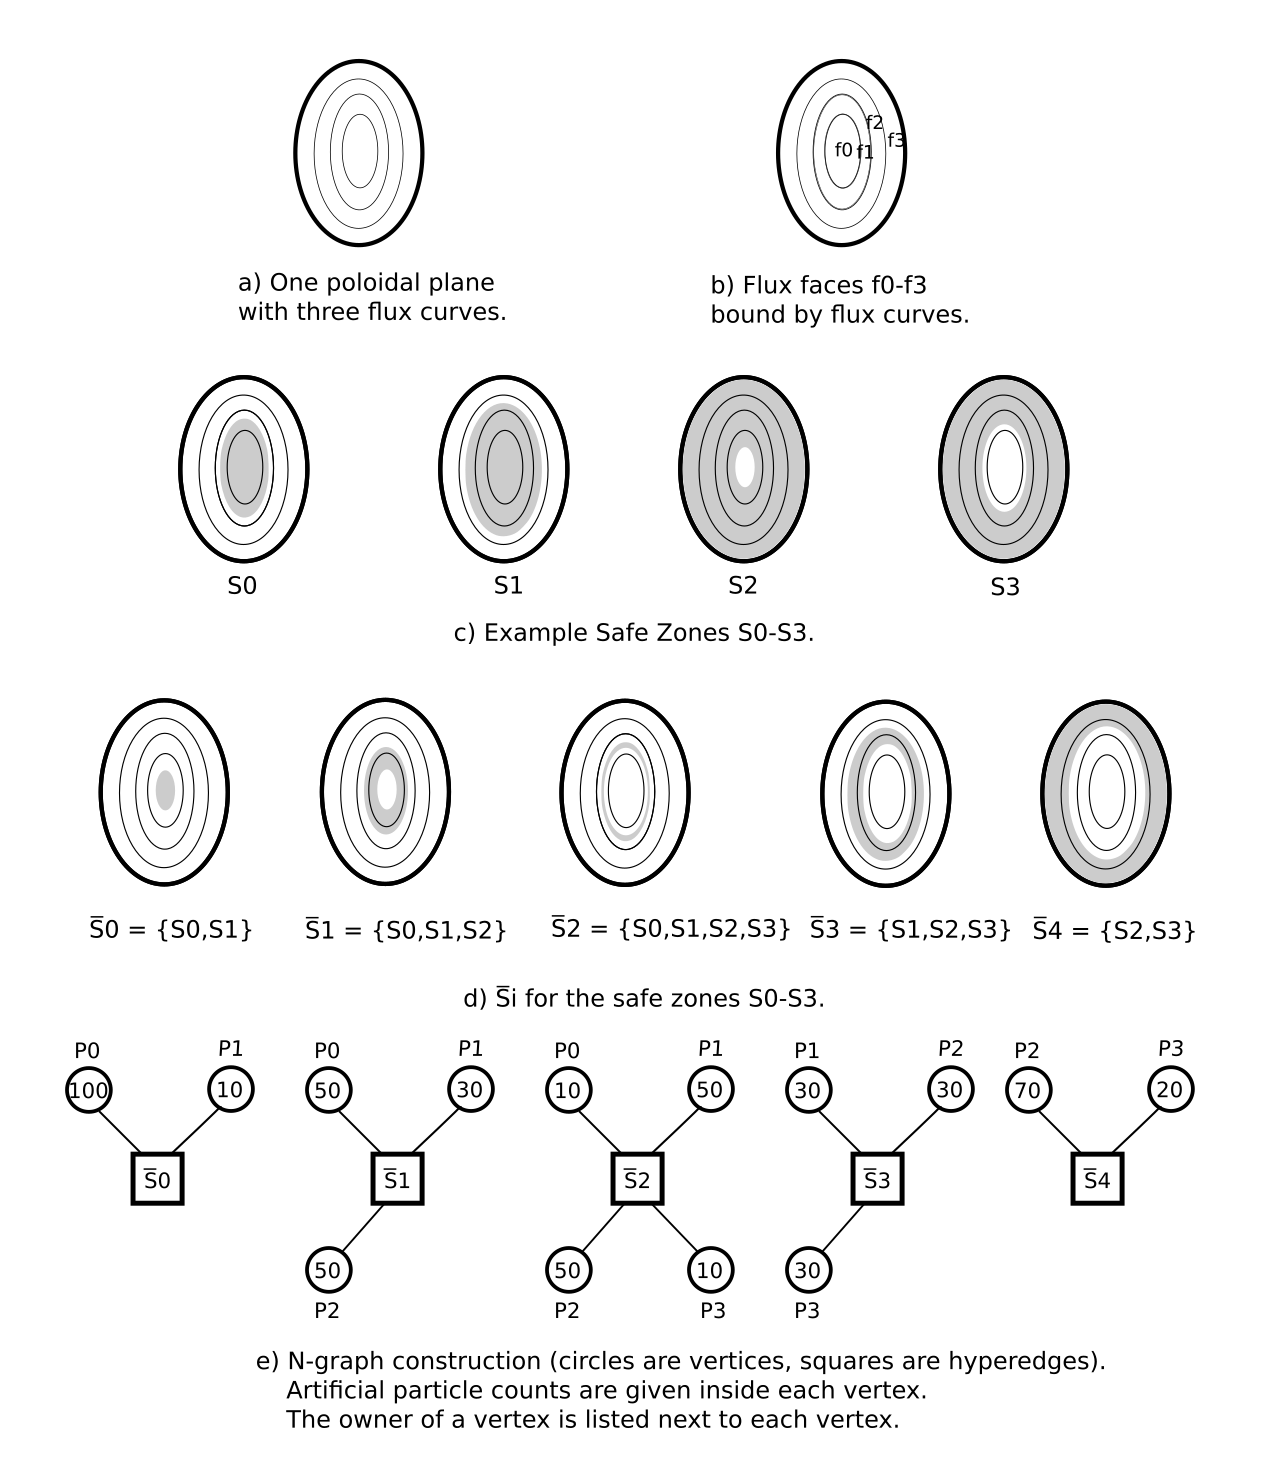
\includegraphics[width=.9\textwidth]{xgcm_ngraph_construction.png}
  \caption{An example of how $\bar{S_i}$ is made from safe zones and the N-graph constructed from them.}
  \label{fig:construct}
\end{figure}

With this formulation we can use some sort of weight diffusion that will
migrate portions of the weight of vertices across the hyperedges to other
processes. {\color{blue} See sections \ref{sec:select} and \ref{sec:migrate}
for details of this method.}


{\color{blue}
  \section{Weight Diffusive Selection}
  \label{sec:select}

  The Sides,Weights, and Targets phases of EnGPar's current diffusive algorithm do not need to be changed for the weight diffuser. However, Selection and Migration will be different since this algorithm will be sending weight instead of vertices. Algorithm \ref{alg:select} provides pseudo code for how selection could be done. This \texttt{RUNSTEP} function would be called iteratively similar to how the current balancer does.

  \begin{algorithm}
    \caption{Seletion Algorithm}
    \label{alg:select}
    \small
    \begin{algorithmic}[1]
      \Procedure{RunStep}{$G$}
      \State Q = an ordering of the owned vertices of $G$.
      \For{$v \in Q$}
      \For{vertex $u$ neighboring $v$}
      \State O = part that owns $u$
      \If{$target\rightarrow has(O) \And sending[O] < target[O]$}
      \State Choose $x$ weight to send from $v$ to $u$
      \Comment{{\tiny $x \le target[O] - sending[O]$}}
      \State
      \Comment{{\tiny$x \le weight(vtx) - sent(vtx)$}}
      \State {\{$v,u,x\} \rightarrow Plan$}
      \State $sending[O] += x$
      \State $sent(vtx) += x$
      \EndIf
      \EndFor
      \EndFor
      \EndProcedure
    \end{algorithmic}
  \end{algorithm}

  \noindent There are two points of this algorithm that we will have to explore what will work best:
  \begin{itemize}
  \item How to order the vertices in the queue
    \begin{itemize}
    \item heaviest/lightiest vertices first?
    \item largets/fewest neighbors first?
    \end{itemize}
  \item How to decide how much weight, $x$, to send in each iteration.
  \end{itemize}

  \section{Weight Migration}
  \label{sec:migrate}

  Given a plan coming out of selection of the form
  $$owned\_vtx \rightarrow \{neighbor\_vertex, weight\}$$
  Algorithm \ref{alg:migrate} will migrate the weight to the neighboring parts.

  \begin{algorithm}
    \caption{Migration Algorithm}
    \label{alg:migrate}
    \small
    \begin{algorithmic}[1]
      \Procedure{Migrate}{$Plan$}
      \For{$\{owned\_vtx,neighbor\_vtx,weight\} \in Plan$}
      \State Send ${neighbor\_vtx,weight} \rightarrow owner(neighbor\_vtx)$
      \State $weight(owned\_vtx) -= weight$
      \EndFor
      \For{each received message $\{owned\_vtx,weight\}$}
      \State $weight(owned\_vtx) += weight$
      \EndFor
      \EndProcedure
    \end{algorithmic}
  \end{algorithm}

  \section{Partition Retrieval}
  Since the partition that EnGPar will report is based on weight being diffused rather than the vertices migrating across parts, the construction of the final parts can be dealt with in several different ways. Two main concerns arise because of this:
  \begin{itemize}
  \item How we should report the partition?
    \begin{itemize}
    \item Do we report just the final weights of each vertex?
    \item Should we give the amount of weight each vertex sent to every other vertex?
    \end{itemize}
  \item How to quickly construct/keep track of this partition structure?
    \begin{itemize}
    \item If only reporting the final weights of each vertex, it is easy to report this in a vtx->weights mapping
    \item If reporting a plan of how much weight to send, this is a nontrivial problem with multiple solutions and approaches that could be taken.
    \end{itemize}
  \end{itemize}
  {
  \color{blue}
  \section{Migration of particles}
  After EnGPar has run a weight diffuser, the resulting partition will
  describe the amount of particles that should exist on each process
  for each set $P_{\bar{S_i}}$. XGCM can select particles to satisfy the weight
  distribution given by EnGPar. Any stategy can be employed to choose
  these particles. One such example is: for each $P_{\bar{S_i}}$, we migrate particles
  that are closer to the safe zone of the target part and prioritize sending
  the further out particles. This strategy should reduce the number of times
  a particle is migrated.
  }
  
}

\section{Other Questions}
Here are some questions that may affect the above idea to a smaller degree.
\begin{enumerate}
\item Do particles have different computational load?
  {\color{red}
  \begin{itemize}
  \item Answer: No.
  \end{itemize}
  }
\item How hard would it be to ``compute'' $T_p$, $\bar{S_i}$, and $P_{\bar{S_i}}$?
\item Does the outside regions (near the X point) mess up any of the assumptions or formulations used here?
\end{enumerate}

\section{Other Pieces to Consider}
\begin{itemize}
\item Should we account for particles that have left the safe regions before or during EnGPar's load balancing?
  {\color{red}
    \begin{itemize}
    \item Particles that have left the safe zone must be migrated to another group before the next push operation can occur. For a given process, we can subtract the number of non-safe particles from the number of safe particles to determine the current load. Ideally, we will execute at most one migration event per push to minimize communication costs.
    \end{itemize}
  }
\item Is it possible to get a good partition using a standard graph partitioning method on this or a similar graph construction.
  {\color{red}
    \begin{itemize}
    \item Yes, but will likely be slower than a diffusive approach. Also doesn't directly support weight diffusion.
    \end{itemize}
  }

  \item This design kind of assumes one process per flux face, which as I understand is not the case. However, we should be able to extend this idea for more processes.
\end{itemize}

\end{document}
